\chapter{Introducción}

\section{Contexto}

Hoy en día se tiende a tener distintos recursos de cómputo en un solo dispositivo, por ejemplo, en un teléfono móvil ya tenemos al menos un procesador y una tarjeta gráfica, pero no tan sólo en el ámbito más cotidiano (aunque no nos demos cuenta), sino que en los más profesionales y especializados está siendo también cada vez más común la heterogeneidad de los recursos de computación en servidores, \textit{clusters} y supercomputadores. 

\par\bigskip

Programar estos dispositivos, que cuentan con esta heterogeneidad no es una tarea sencilla, un procesador no se programa de la misma manera que un acelerador, ni dos aceleradores tienen por qué programarse de la misma manera, existen una gran variedad de modelos de programación que nos brindan estas facilidades pero esta gran variedad se torna abrumadora y a veces repercute en la portabilidad de las aplicaciones. Es por esto que nos hemos decidido a hacer este proyecto, para mejorar en la medida de lo posible la facilidad de desarrollo y portabilidad de una aplicación en estas plataformas cada vez más complejas.

\par\bigskip

Si se facilita a la comunidad este tipo de programación, no solo habría una disminución del esfuerzo a realizar por parte del programador (hasta ahora, abismal), si no que mejoraría el desempeño de las aplicaciones que utilizasen todos los recursos que hay a su disposición en una máquina. Esto motiva la realización del proyecto, que pretende facilitar la gestión de estos recursos de computación en entornos distribuidos, brindando un método robusto y eficiente para programar aplicaciones en estos entornos.

\par\bigskip

Este proyecto es un Trabajo de Fin de Grado del Grado en Ingeniería Informática, especializado en el área de Ingeniería de Computadores. El grado es impartido por la \textit{Facultat d'Informàtica de Barcelona (FIB)} centro perteneciente a la \textit{Universitat Politècnica de Catalunya (UPC)}. 
\par\bigskip

El proyecto se ha desarrollado conjuntamente con el \textit{Barcelona Supercomputing Center (BSC)}, hemos estudiado como integrar los modelos de programación \textit{COMPSs} y \textit{OmpSs} para alcanzar este objetivo, se ha implementado y evaluado un prototipo.
%Indagar en cuales son estas caracteristicas? 

\subsection{Actores}

Los actores en este proyecto son las personas que tomen parte en él, ya sea de manera directa o indirecta. Con esto quiero decir, que tanto las personas que han tomado parte en el desarrollo \textit{per se} como las personas que se nutran de este, son los actores.

\begin{itemize}
 \item \textbf{Desarrollador:} La figura del desarrollador \textbf{es} la persona que ha trabajado de manera más directa en el proyecto. En este proyecto únicamente hay un desarrollador que ha elaborado la documentación que leerás a continuación y ha dado forma a los objetivos tangibles del proyecto.  
 \item \textbf{Director y codirector:} Pese a que el desarrollador ha tenido el papel principal en el proyecto, el director y el codirector han guiado a este en el camino abierto que es el desarrollo del proyecto. Periódicamente ha habido reuniones de seguimiento donde se han supervisado las actividades del proyecto y su correcta realización.
 \item \textbf{Barcelona Supercomputing Center:} De manera directa el centro otorga al desarrollador un lugar de trabajo y un equipo informático. Por otra parte, cuenta con el soporte por parte de los equipos de desarrollo de \textit{COMPSs} (del cual forma parte el desarrollador) y de \textit{OmpSs} para cualquier incidencia relacionada con su \textit{software} y derivados.
 \item \textbf{Beneficiarios:} El proyecto facilita el desarrollo de aplicaciones paralelas en entornos heterogéneos distribuidos, de manera que se espera que los beneficiarios sean cualquier desarrollador de esta, sea de la organización que sea.
\end{itemize}

\section{Estado del arte}

Existen muchos modelos de programación, véanse \textit{OpenMP}\cite{dagum1998openmp}, \textit{OmpSs}\cite{duran2011ompss}, \textit{MPI}\cite{walker1996mpi}, \textit{COMPSs}\cite{badia2015comp} y un largo etcétera. De alguna manera el objetivo en común fue y es aprovechar los cada vez más abundantes recursos en las máquinas, que finalmente no sólo han crecido en abundancia si no en diversidad. La filosofía sigue siendo la misma, sacar el mayor rendimiento posible a nuestras máquinas. 
\par\bigskip

Para esto son necesarios modelos de programación que nos den la posibilidad de utilizar los recursos y nos ayuden a explotar la posible sinergia entre estos en ciertas aplicaciones. 
\par\bigskip

La diferencia más elemental entre los modelos, es en como se gestiona la memoria, o más bien cómo se estructura en el modelo.

\begin{itemize}
\item \textbf{Memoria compartida:} En un modelo con memoria compartida como \textit{OpenMP} o \textit{OmpSs}, el paralelismo se consigue a través de hilos o \textit{threads} que ejecutan porciones de código. Los \textit{threads} dentro de una aplicación comparten la memoria, es decir que el espacio de direcciones es el mismo para todos. De esta manera cualquier modificación será inmediatamente visible en el resto de \textit{threads}.
\item \textbf{Memoria distribuida:} En un modelo con memoria distribuida esta no es compartida entre los procesos que llevan a cabo el cómputo (en memoria compartida hilos), esto es que tienen su propio espacio de direcciones y en caso de necesitar un dato en concreto se debe efectuar una comunicación. Existen distintas formas de implementar un modelo con memoria distribuida.
		\subitem \textbf{Paso de mensajes:} \textit{MPI} es un modelo de programación con memoria distribuida por paso de mensajes (\textit{Message Passing Interface}) , cada proceso goza de un espacio de direcciones único y el programador es consciente de esto cuando programa la aplicación, es encargado de reservar la memoria y también de efectuar las comunicaciones, todo esto mediante llamadas a una \textit{API}.

		\subitem \textbf{Memoria global:} A diferencia del anterior, el programador tiene una visión global de la memoria, pero cada proceso tiene su propio espacio de direcciones, en caso de que intente acceder a memoria perteneciente al espacio de direcciones de otro proceso, se hará la transferencia de uno a otro. Modelos de programación que hagan uso de memoria global son \textit{UPC}\cite{berkupc}, y \textit{GASPI}\cite{grunewald2013gaspi} y \textit{COMPSs}\cite{badia2015comp}.
 
		\subitem \textbf{Entornos heterogéneos:} La memoria se encuentra dividida entre la correspondiente al \textit{host} (el procesador) y el \textit{device} (el dispositivo, que será un acelerador), para que este dispositivo compute hay que enviarle todos los datos que vaya a necesitar, por lo que la memoria entre el procesador y el acelerador está distribuida, modelos que hagan uso son \textit{CUDA}\cite{luebke2008cuda} y \textit{OpenCL}\cite{stone2010opencl}, por ejemplo.
\end{itemize}

\par\bigskip
La integración de los modelos propuestos \textit{COMPSs} y \textit{OmpSs} nos otorgará la posibilidad de utilizar todos los recursos de la máquina, e incluso de otras máquinas, ya que estaríamos usando la conjunción de un modelo basado en memoria compartida con uno en memoria distribuida, a continuación se ahonda en las características de ambos.

\section{COMPSs}

\textit{COMPSs} está desarrollado por el grupo \textit{Workflows and Distributed Computing} que pertenece al departamento de \textit{CS - Computer Science}.
\par\bigskip

\textit{COMPSs} es un modelo de programación para entornos distribuidos basado en la generación de tareas. El objetivo es hacer más sencilla la programación de aplicaciones y su ejecución en entornos distribuidos (clústers y \textit{clouds}, por ejemplo). La generación de tareas la efectua un programa principal ejecutado en secuencial donde las tareas se especifican mediante la anotación de las funciones que se deseen.   

\par\bigskip

El modelo está dotado de un sistema de \textit{runtime} que coexiste con la aplicación. A medida que el programa principal encuentra las tareas y las envía al \textit{runtime} este genera un grafo de tareas y se detectan las dependencias entre estas para ejecutarlas en el orden correcto. Dado que está preparado para ejecutarse en entornos distribuidos el \textit{runtime} también detecta cuando son necesarias transferencias entre nodos.

\subsection{Modelo de programación} 
\label{compss_pm}

El \textit{runtime} de \textit{COMPSs} está implementado en \textit{Java} por lo cuál se soporta dicho lenguaje, además se desarrollaron los \textit{bindings} de \textit{Python}\cite{tejedor2017pycompss} y \textit{C/C++} para facilitar el portaje de aplicaciones en estos lenguajes a \textit{COMPSs}. 
\par\bigskip

En este proyecto centraremos nuestros esfuerzos en \textit{C} y \textit{C++}. Para desarrollar una aplicación de \textit{COMPSs} en \textit{C/C++} necesitamos el programa principal (ejecutado en secuencial), una interfaz que especificará las funciones que \textit{a posteriori} serán tareas, y el código que realmente implementan estas tareas. 
\par\bigskip

Veamos en orden de enumeración ejemplos de los componentes de una aplicación.

%EJEMPLO INTERFACE
\begin{minipage}{\linewidth}
\begin{lstlisting}[caption={Interfaz de la aplicación 'ejemplo'.},captionpos=b, label={lst:ejemplo.idl}, style=idlstyle]
interface ejemplo {
    void funcionEjemplo(in int a, out int[a] array_a);
};
\end{lstlisting}
\end{minipage}

La interfaz de la imagen superior define una función llamada \textit{funcionEjemplo} con un parámetro de entrada y uno de salida, las palabras clave \textit{in} y \textit{out} respectivamente otorgan estas propiedades a los parámetros, también se puede utilizar \textit{inout}, el parámetro será de entrada y salida. Cualquier llamada a la función será ejecutada como tarea.\smallskip

%EJEMPLO MASTER CODE
\begin{minipage}{\linewidth}
\begin{lstlisting}[caption={Fracción del código del programa principal}, captionpos=b, label={lst:ejemplo.cc}, language=C++]
    compss_on();

    int a = 10;
    int* array_a;

    funcionEjemplo(a, array_a);

    compss_wait_on(array_a);

    compss_off();
\end{lstlisting}
\end{minipage}

Esta imagen muestra el código del programa principal. Es tan sencillo como prometía, encendemos el \textit{runtime} de \textit{COMPSs}, preparamos los parámetros de la función, ejecutamos y finalmente esperamos a los parámetros de salida y apagamos el \textit{runtime}. \smallskip

\begin{minipage}{\linewidth}
\begin{lstlisting}[caption={Implementación de la función 'funcionEjemplo'}, captionpos=b, label={lst:ejemplo-functions.cc}, language=C++]
void funcionEjemplo(int a, int array_a[]) {
    for (int i = 0; i < a; ++i) {
        array_a[i] = a;
    }
}
\end{lstlisting}
\end{minipage}

Las tareas se implementan como funciones que serán ejecutadas por los \textit{workers}. Salvo convenciones en los nombres de los ficheros para hacer la compilación de la aplicación esto es todo lo necesario para desarrollar una aplicación en \textit{COMPSs} de \textit{C/C++}.

\begin{comment}
\subsubsection{Compilación}

Para compilar la aplicacion en \textit{COMPSs} de \textit{C/C++}, 

\begin{figure}[H]
    \centering
    \caption{Proceso de compilado de una aplicación COMPSs C/C++}
%    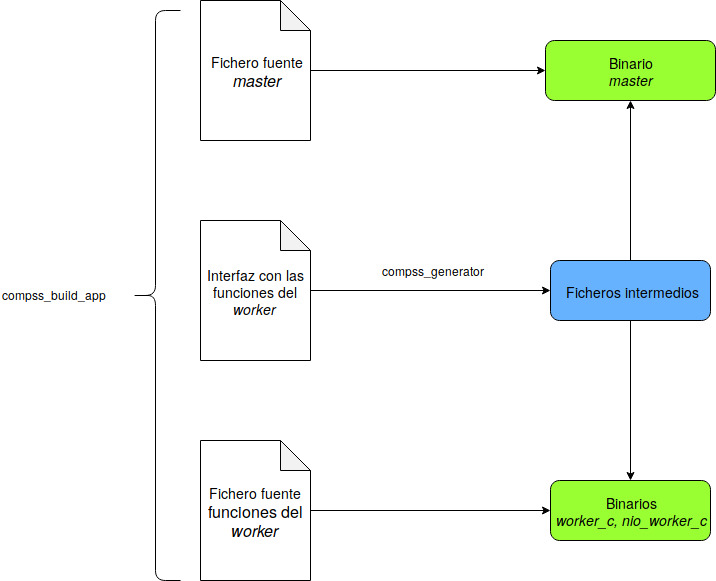
\includegraphics[width=\textwidth]{proceso_compilado.jpg}
    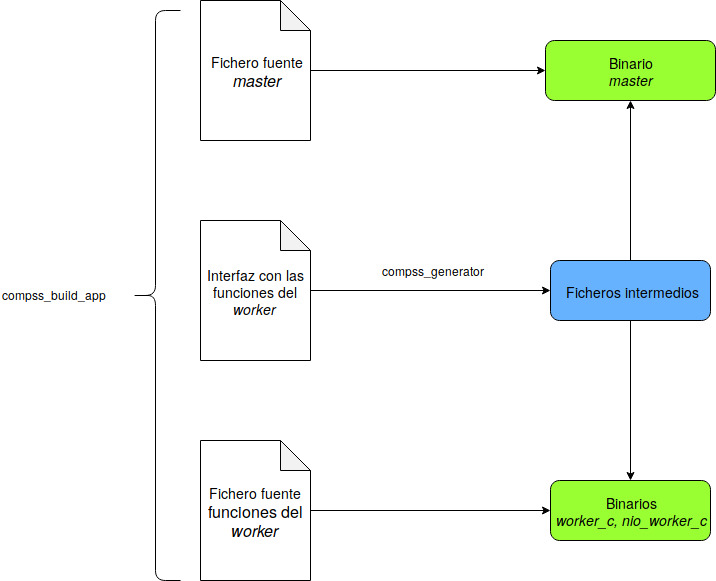
\includegraphics[scale=0.5]{proceso_compilado.jpg}
    \label{fig:proceso_compilado}
\end{figure}
\end{comment}

\subsection{Modelo de ejecución\label{modeloejecucion}}

El modelo de ejecución es sencillo, muy similar al modelo \textit{thread-pool}, al iniciar el \textit{runtime} se levanta el \textit{master} y un conjunto de \textit{workers}, a medida que se vayan generando tareas se estudiará qué \textit{workers} están libres y si cumplen los requisitos para ejecutar dicha tarea, y en ese caso la ejecutarán. 

\begin{figure}[H]
    \centering 
    \caption{Modelo de ejecución, basado en la aplicación 'ejemplo'.}
    %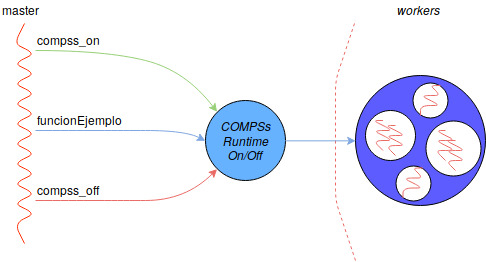
\includegraphics[width=\textwidth]{sta-masterworker.jpg}
    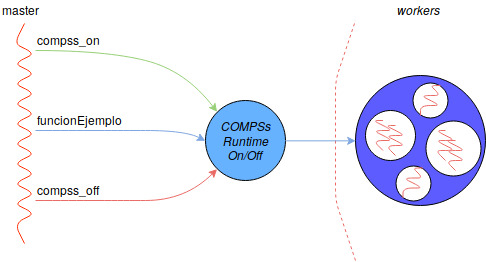
\includegraphics[scale=0.75]{sta-masterworker.jpg}
    \label{fig:masterworker_pool}
\end{figure}

La imagen muestra lo que sucede al ejecutar la aplicación de ejemplo de la sección \ref{compss_pm}, las líneas rojas curvas indican procesos (o bien \textit{threads}), lo importante sucede entre las flechas etiquetadas como compss\_on y compss\_off, la ejecución de la tarea. Se pide ejecutar la tarea funcionEjemplo al \textit{runtime} de \textit{COMPSs} y se decide en qué \textit{worker} se ejecutará. Hasta aquí podríamos pensar que es indéntico al \textit{thread-pool}. Nótese, que esto no es así, por el hecho de que no tenemos por qué hablar de una misma máquina, sino que pueden ser máquinas distintas, como se puede ver en el grupo de ordenadores de la imagen. 
\par\bigskip

En \textit{C/C++} existen dos tipos de \textit{worker}, uno \textbf{no persistente} y otro \textbf{persistente}. 

\begin{itemize}
 \item \textbf{No persistente:} Para cada tarea que se quiere ejecutar en uno de estos workers se debe crear el \textit{thread} y unas \textit{pipes} para hacer \textit{Inter-process communication} (IPC). %No sé si indagar en qué se pasa por las pipes, hmmm... qué se pasa por las pipes?
 \item \textbf{Persistente:} Este tipo de \textit{worker} se levanta una vez al inicio de la aplicación y espera recibir las tareas a ejecutar.
\end{itemize}


\section{OmpSs}

\textit{OmpSs} es desarrollado por el grupo \textit{PM - Programming Models}, perteneciente también al departamento de \textit{CS - Computer Science}.
\par\bigskip

\textit{OmpSs} es un modelo de programación que intenta explotar el paralelismo de las aplicaciones de una manera sencilla y aprovechando al máximo los recursos de la máquina\cite{duran2011ompss}. 
\par\bigskip
El nombre del modelo proviene de \textit{OpenMP} y \textit{StarSs} (modelo que desarrolló el \textit{BSC}), este integra funcionalidades presentes en ambos. Por parte de \textit{OpenMP} se quiere tomar la facilidad de paralelizar una aplicación secuencial insertando pragmas, y de \textit{StarSs} el modelo de ejecución basado en un \textit{thread-pool} y que permite la ejecución de código en más recursos que únicamente el procesador, es decir, que ofrece fácil gestión del resto de recursos de cómputo (\textit{GPUs}, \textit{FPGAs}, ...)\cite{sainz2014leveraging}\cite{filgueras2013heterogeneous}.

\subsection{Modelo de programación y ejecución}

El modelo de programación de \textit{OmpSs} se basa en la generación de tareas sencillamente insertando pragmas en código secuencial y a su vez facilitando la gestión de recursos heterogéneos. Veamos un pequeño ejemplo que muestre estas facultades.

\begin{minipage}{\linewidth}
\begin{lstlisting}[caption={Multiplicación de un bloque de una matriz utilizando GPUs.}, captionpos=b, label={lst:ompssmatmul.cc}, style=JStyle]
for (int i = 0; i < N; ++i) {
    for (int j = 0; j < N; ++j) {
        for (int k = 0; k < N; ++k) {
            #pragma omp target device(cuda) \
                               copy_deps    \
                               ndrange(2,N,N,32,32)
            #pragma omp task inout([N*N]C) in([N*N]A, [N*N]B)
            multiply_partitions_GPU(A[i*N+k], 
                                    B[k*N+j], 
                                    C[i*N+j], 
                                    n);
        }
    }
}
\end{lstlisting}
\end{minipage}

El código muestra una multiplicación de matrices por bloques. Con el primer pragma se indica que el dispositivo objetivo es una tarjeta gráfica que soporte \textit{CUDA}, y el segundo la declaración de una tarea y el tamaño de los bloques junto a las dependencias de esta.
\par\bigskip

El modelo de ejecución consiste en un \textit{thread-pool}, es decir, al generar tareas se escogerán \textit{threads} del \textit{pool} (entendámoslo como un conjunto de \textit{threads}) para ejecutarlas.
\par\bigskip

Cabe decir que para compilar una aplicación de \textit{OmpSs}, se utiliza el compilador \textit{source-to-source Mercurium} y el runtime \textit{Nanos++} para gestionar el paralelismo, es decir, la creación de tareas, sincronización entre estas, etc.

\section{Trabajo previo} 
\label{sec:compssompss}

Actualmente existe la posibilidad de desarrollar aplicaciones que utilicen \textit{OmpSs} dentro de \textit{COMPSs}. 
\par\bigskip
Para poder interactuar con el \textit{runtime} de \textit{OmpSs} \textit{Nanos++}, necesitamos gestionarlo nosotros manualmente o bien utilizar los \textit{pragmas} que nos propone el modelo de programación y compilar con \textit{Mercurium}. Entonces, asegurándonos de registrar los \textit{workers} en el \textit{runtime} y compilando su código fuente con \textit{Mercurium} aseguramos la interacción con el \textit{runtime} y por lo tanto la integración de ambos modelos.

Es posible desarrollar aplicaciones, pero con ciertas limitaciones. Dado que el worker \textit{no persistente}, se debe levantar para cada tarea conseguimos aislar las tareas entre sí, cada tarea tendrá un \textit{runtime} de \textit{OmpSs} para el mismo, pero este mismo motivo añade mucho \textit{overhead} para la granularidad de las tareas de \textit{OmpSs}. El \textit{worker persistente} carece del \textit{overhead} de poner en marcha el \textit{runtime} de \textit{OmpSs} pero también pierde la característica de aislar cada tarea del resto. 
\par\bigskip
El factor de aislamiento se vuelve todavía más crítico cuando en \textit{OmpSs} efectuar un \textit{taskwait} (\textit{pragma} que espera hasta que las tareas acaben) conlleva a que la espera se haga sobre todas las tareas de \textit{OmpSs} que estén en el \textit{runtime} por lo cual si no contamos con el aislamiento esperaremos a todas, hayan sido creadas o no por la misma tarea de \textit{COMPSs}. Para solucionarlo hay que efectuar accesos concurrentes sobre los datos que estemos tratando y hacer que el \textit{taskwait} tenga como dependencia esos datos, así no esperaremos a absolutamente todas las tareas.
\par\bigskip
Estos problemas pretenden arreglarse integrando \textit{OmpSs-2}, que ofrece un \textit{runtime} nuevo llamado \textit{Nanos6} y nuevas características que vienen con este cambio como por ejemplo:

\begin{itemize}
\item \textbf{Liberación de las dependencias:} Las dependencias en esta versión se liberan de manera temprana, es decir, una vez una tarea acaba con un dato lo notifica al \textit{runtime} y este se encarga de notificar a las tareas que quedan libres de esta dependencia.
 \item \textbf{Relajación de las dependencias:} Ahora se pueden utilizar nuevos pragmas para determinar dependencias más suaves, no tan estrictas como en la versión anterior.
 \item \textbf{Ejecución de funciones de manera asíncrona:} La \textit{API} del nuevo \textit{runtime} \textit{Nanos6} permite ejecutar de manera asíncrona funciones en forma de tarea a partir de un puntero a una función, este método proporciona aislamiento del resto de tareas.
\end{itemize}

Hemos listado las que de alguna manera han sido clave para el proyecto, \textit{OmpSs-2} implementa muchas otras mejorías a parte de estas\cite{OmpSs2reference}. El proyecto estudia en los capítulos \ref{sec:estudiopreviorend} y \ref{sec:estudiorend} si los problemas planteados han sido solucionados y el rendimiento que desempeña la nueva integración.

\section{Alcance del proyecto}

En esta sección se declaran las intenciones del proyecto (qué se pretende hacer), mediante una serie de requerimientos que harán que el proyecto pueda ser acabado con éxito, y unos objetivos que marcarán el desarrollo de este. También los posibles riesgos que surjan (y las soluciones de estos) y la metodología de trabajo que se llevará a cabo.

\subsection{Requerimientos}

 Los requerimientos necesarios para este proyecto son:

\begin{itemize}
 \item La nueva integración con \textit{OmpSs-2} no debe romper la actual compatibilidad con \textit{OmpSs}.
 \item El rendimiento de las aplicaciones desarrolladas con \textit{COMPSs+OmpSs-2} debe mejorar.
 \item Todas las modificaciones sobre \textit{COMPSs} deben ajustarse al grupo de \textit{Workflows and Distributed Computing}.
 \item Cualquier requerimiento impuesto (o aconsejado) por el \textit{BSC} formará parte de esta lista.
  
\end{itemize}

\subsection{Objetivos}

El objetivo principal de este proyecto es reformular la integración de \textit{COMPSs} con \textit{OmpSs} para solucionar los problemas actuales, ya sea integrándolo de nuevo pero esta vez con \textit{OmpSs-2} o bien idear otra manera de resolver las problemáticas. La siguiente lista muestra la posible descomposición de objetivos:

\begin{itemize}
  \item Aprender a utilizar la API (\textit{Application Programming Interface}) de \textit{Nanos6}.
  \item Eliminar o bien reducir las problemáticas planteadas en la sección   \ref{sec:compssompss}.
  \item Mejorar la gestión de recursos heterogéneos en las aplicaciones desarrolladas en \textit{COMPSs} integrando \textit{OmpSs-2}.
  \item En caso de conseguir el resto de objetivos plantear la integración en \textit{Java} y \textit{Python}.
\end{itemize}

\subsection{Riesgos}

Durante el desarrollo del proyecto pueden surgir problemas, para mejorar la reacción ante ellos listaremos los posibles riesgos y las respectivas soluciones.

\subsubsection{Problemas con el material de desarrollo}

Se podría romper el equipo en el cual se desarrolla el proyecto, pongamos que de una pantalla, un teclado y un ordenador se rompe el último. Se perdería todo el avance del proyecto, incluso documentación.
\par\medskip

\textbf{Solución:} Pese a que la pérdida del ordenador es importante, todo el código del proyecto será subido al \textit{GitLab} de \textit{WDS}, y la documentación al \textit{GitHub} personal del desarrollador, por lo cual se podría recuperar todo el  proyecto.

\subsubsection{Problemas con los clústers y supercomputadores}

Si por casualidad, caen los clústers y supercomputadores en los cuales se medirá el rendimiento del proyecto, se pararía la obtención de las métricas. 
\par\medskip

\textbf{Solución:} En este caso, como no resultaría lo mismo ejecutarlo en local en mi ordenador, debería optar por realizar otras tareas hasta que el equipo del \textit{BSC} solucione los inconvenientes.

\subsubsection{Aparición de errores en la implementación}

Cualquier proyecto esta lleno de errores en la implementación, hay que saber encontrarlos y solucionarlos lo más rápido posible, pero puede entorpecer el proyecto.
\par\medskip

\textbf{Solución:} Activaremos los \textit{flags} de \textit{debug} para poder evitar el mínimo error y en caso de su aparición utilizaremos \textit{gdb} (\textit{GNU Debugger}) para encontrarlo.

\subsubsection{Problemas con OmpSs/OmpSs-2}

Dado que se realizará una integración de otro proyecto del \textit{BSC} el desarrollador puede encontrarse con dificultades relacionadas con este a lo largo del proyecto.
\par\medskip

\textbf{Solución:} Después de haber intentado solucionarlo por sus propios medios se pondrá en contacto con el grupo de \textit{Programming Tools} con la descripción del error e intentos de solucionarlo.

\subsection{Metodología}

Para decidir la metodología a utilizar, hay que tener en cuenta que el proyecto consta únicamente de tres personas que se envolverán en él. El desarrollador, que hará todo el desarrollo tangible, el director y el co-director. 
\par\bigskip

La metodología que más se ciñe a las características del ``equipo'' es la iterativa. Consiste en planear las tareas a realizar y hacer una predicción de qué se conseguirá hacer en cortos periodos de tiempo llamados iteraciones. Además de estas predicciones, se consultará el estado del proyecto a menudo y se realizarán las tareas, una vez acabada una iteración empezará la siguiente, así hasta finalizar el proyecto.
\par\bigskip
Esta metodología nos permitirá reaccionar rápidamente a los imprevistos, además de hacer un bueno monitoreo del estado del proyecto, por lo cual se ha decidido emplearla.

\subsubsection{Herramientas}

Para efectuar el seguimiento del proyecto junto a mi director y codirector, se empleará un \textit{workspace} de \textit{Slack} para las comunicaciones directas (decidir dónde y cuándo hacer las reuniones por ejemplo), y \textit{Trello} para gestionar las tareas a desempeñar en cada iteración. Como ya se ha mencionado anteriormente, para el control de versiones del proyecto, código y documentación se utilizará respectivamente \textit{GitLab} y \textit{GitHub}.